\documentclass[tikz,border=2pt]{standalone}
\usepackage{amsmath,amssymb}
\usetikzlibrary{arrows.meta,decorations.pathreplacing}
\begin{document}
% Alternating up periods Z_k (mean m_f = 1/lambda_f) and repairs R_k (mean E[R]); the ends of the
% repairs T_1, T_2, T_3 split time into cycles, and by the renewal reward theorem the long-run
% fraction of up time is A = m_f/(m_f + E[R]).
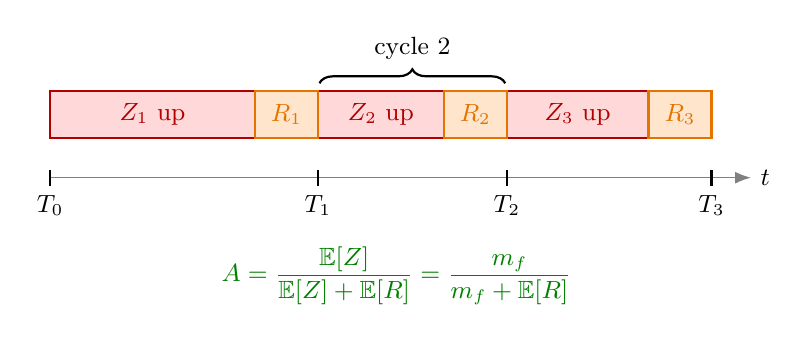
\begin{tikzpicture}[font=\small, >={Latex[length=2mm]}, x=1cm, y=1cm]
  \tikzset{up/.style={draw=red!70!black, fill=red!15, thick},
           outage/.style={draw=orange!90!black, fill=orange!20, thick}}
  \foreach \a/\b/\k in {0/2.6/1, 3.4/5.0/2, 5.8/7.6/3} {
    \draw[up] (\a,0) rectangle (\b,0.6);
    \node[red!70!black] at ({(\a+\b)/2},0.3) {$Z_{\k}$ up};
  }
  \foreach \a/\b/\k in {2.6/3.4/1, 5.0/5.8/2, 7.6/8.4/3} {
    \draw[outage] (\a,0) rectangle (\b,0.6);
    \node[orange!90!black] at ({(\a+\b)/2},0.3) {$R_{\k}$};
  }
  % cycle ends
  \draw[->, gray] (0,-0.5) -- (8.9,-0.5) node[right, black] {$t$};
  \foreach \t/\k in {0/0, 3.4/1, 5.8/2, 8.4/3} {
    \draw[thick] (\t,-0.6) -- (\t,-0.4);
    \node[anchor=north] at (\t,-0.6) {$T_{\k}$};
  }
  \draw[decorate, decoration={brace, amplitude=5pt}, thick] (3.42,0.7) -- (5.78,0.7)
    node[midway, above=5pt] {cycle 2};
  \node[green!50!black, anchor=north] at (4.4,-1.25)
    {$A=\dfrac{\mathbb{E}[Z]}{\mathbb{E}[Z]+\mathbb{E}[R]}=\dfrac{m_f}{m_f+\mathbb{E}[R]}$};
\end{tikzpicture}
\end{document}
